% Die Beamer-Klasse unterstützt folgende Optionen, die von
% besonderem Interesse sind (alle Standardoptionen werden
% ebenfalls unterstützt; siehe beamer-Basisdokumentation):
% 
%%%%%%%%%%%%%%%%%%%%%%%%%%%%%%%%%%%%%%%%%%%%%%%%%%%%%%%%%%%%%%%
% aspectratio: Seitenverhältnis des resultierenden Dokuments
% (Achtung: Aufgrund der Designvorgaben ergeben sich unterschiedliche
% Größen der effektiv nutzbaren Textblöcke)
%
% Standardeinstellung: 'aspectratio=43'
%
% Mögliche Einstellungen:
% 'aspectratio=43'   (4:3)
% 'aspectratio=169'  (16:9)
% 'aspectratio=1610' (16:10)
% 
%%%%%%%%%%%%%%%%%%%%%%%%%%%%%%%%%%%%%%%%%%%%%%%%%%%%%%%%%%%%%%%
% fontsize: Basisschriftgröße (Größen für Überschriften etc. werden
% aus dieser Basis automatisch abgeleitet)
%
% Standardeinstellung: '22pt' (entspricht den Design-Vorgaben; sehr groß!)
%
% Mögliche Einstellungen:
% '8pt', '9pt', '10pt', '11pt', '12pt', '14pt', '16pt',
% '17pt','20pt','22pt', '24pt', '26pt', '28pt'

\documentclass[aspectratio=169,16pt,xcolor=table]{beamer}

% Der OTHR-Theme unterstützt folgende Optionen:
% 
%%%%%%%%%%%%%%%%%%%%%%%%%%%%%%%%%%%%%%%%%%%%%%%%%%%%%%%%%%%%%%%
% department: (Wahl der Abteilung/Fakultät)
%
% default: 'OTHR'
%
% Mögliche Einstellungen:
% 'FakA', 'FakAM', 'FakB', 'FakBW', 'FakEI', 
% 'FakIM', 'FakM', 'FakS', 'ZWW', 'IPF',
% 'SappZ', 'KNB', 'ReMIC', 'LFD', 'LAS3',
% 'DK0PT', 'LBM', 'LeanLab', 'LFT', 'LFW',
% 'LMP', 'LMS', 'LRT', 'LWS', 'RRRU',
% 'RST', 'CEEC', 'FEM', 'IST'
%%%%%%%%%%%%%%%%%%%%%%%%%%%%%%%%%%%%%%%%%%%%%%%%%%%%%%%%%%%%%%%%%
% headerMode: Aussehen und Inhalt der Kopfleiste
%
% Standardeinstellung: 'full'
%
% Mögliche Einstellungen:
% 'full', 'frametitle', 'frametitleSection'
% 

%%%%%%%%%%%%%%%%%%%%%%%%%%%%%%%%%%%%%%%%%%%%%%%%%%%%%%%%%%%%%%%%%
% Binäre Schalter (können angegeben oder nicht angegeben werden;
% Standardeinstellung: Nicht angegeben)
%
%%%%%%%%%%%%%%%
% navbar: Navigationssymbole anzeigen (Seite vor/zurück, Kapitel vor/zurück etc.)

% pageNumbers: Seitennummerierung

% blackFont: Nur schwarze Schriftfarbe verwenden (ansonsten: Fakultätsfarben)

% frametitleCenter: Titel in der Kopfzeile zentrieren (ansonsten: rechtsbündig)

\usetheme[department=FakIM,pageNumbers]{OTHR}

% Inhaltsspezifische Zusatzpakete laden 
\usepackage[ngerman]{babel}
\usepackage[utf8]{luainputenc}
\usepackage{lipsum}
\usepackage{graphicx}
\graphicspath{ {./img/} }
\usepackage{amsmath}
\usepackage{adjustbox}
\usepackage{xcolor}
\usepackage{ulem}
\usepackage[usestackEOL]{stackengine}
\usepackage{hyperref}
\usepackage{biblatex}
\usepackage{breakcites}
\usepackage{etoolbox}

\renewcommand\bibfont{\tiny}
\addbibresource{ref.bib}

\patchcmd{\thebibliography}{\footnotesize}{\tiny}{}{}

% this adds the content table for each section
\AtBeginSection[]
{
  \begin{frame}
    \frametitle{Inhalt}
    \tableofcontents[currentsection]
  \end{frame}
}

\date{15. Januar 2024}

\begin{document}

\begin{frame}{YouTube Video Vorschau}
    \centering
    \href{https://www.youtube.com/watch?v=PLk8Pm_XBJE&t=612s}{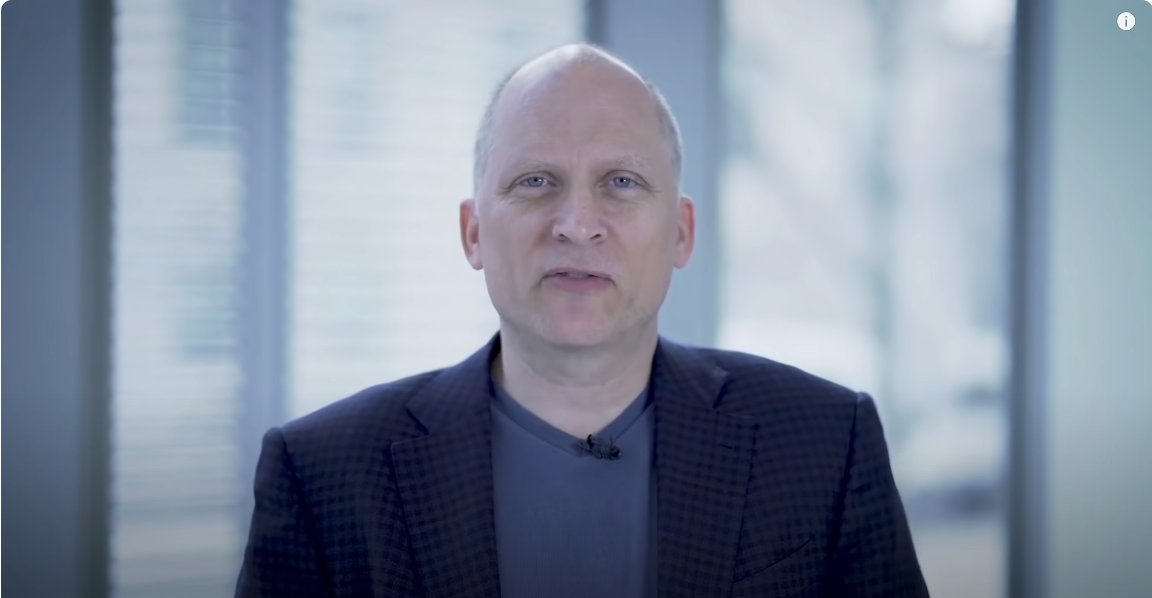
\includegraphics[width=0.8\linewidth]{pictures/Video_Vorschau.png}}
    \vspace{-0.2cm}
    \begin{flushleft}
        \tiny Quelle: \url{https://www.youtube.com/watch?v=PLk8Pm_XBJE}, zuletzt besucht am 12.12.2023
    \end{flushleft}
\end{frame}

\title{Transhumanismus}
\subtitle{Fortschritt oder Dystopie?}
\author{Marcel Ott, Nicolas Zander, Lorenz Branner, Severin Bittl, Thomas Gailinger}
\institute{Ethik in der Informatik}

\maketitle

%\begin{frame}
%	\frametitle{Inhaltsverzeichnis}
%	\tableofcontents
%\end{frame}

\section{Einleitung}
\subsection{Begriffserleuterungen}
\begin{frame}
	\frametitle{Begriffserleuterungen}
	\begin{itemize}
	  \item Transhumanismus
    \begin{itemize}
      \item Ausschöpfung der natürlichen menschlichen Grenzen mit Wissenschaft~\cite{Merzlyakov2022}\\
      => Beibehaltung der Grundform des Menschen
    \end{itemize}
	\item Posthumanimus
    \begin{itemize}
      \item Überwindung der menschlichen Grenzen~\cite{Merzlyakov2022}\\
      \item Mensch ist eine Sackgasse und Cyborg wird als nächster Schritt der Evolution angesehen~\cite{Merzlyakov2022}\\
      => Grundform des Menschen wird abgeschafft
    \end{itemize}
	\item Cyborg
    \begin{itemize}
      \item Integriertes System aus menschlichen und maschinellen Teilen~\cite{warwick2000cyborg}
    \end{itemize}
	\end{itemize}
  \scriptsize Grenzen zwischen Transhumanismus und Posthumanismus sind jedoch fließend werden, aber oft synonm verwendet, was jedoch aufgrund der Unterschiede von vielen Forschern kritisiert wird~\cite{Merzlyakov2022}
\end{frame}

\subsection{Was ist normal?}
\begin{frame}
  \frametitle{Was ist normal?}
  Dr. Anette Breczko: Die Überwachung biotechnologischer Möglichkeiten erfordert zweifellos eine Unterscheidung zwischen ``therapeutischen'' und ``Verbesserungs''-Aktivitäten~\cite{breczko2021human}
  
  \vspace{12pt}
  \textbf{Zentrale Frage hierfür:} Was ist normal? 
\end{frame}

\begin{frame}
	\frametitle{Was ist normal?}
  \textbf{Was ist normal?}

  \vspace{12pt}
  \small Erscheint intuitiv als triviale Frage mit folgenden Antworten:
	\begin{itemize}
	  \item Statischer Durchschnitt
	  \item Mehrheit
	  \item Herrschende Klasse z. B. POC als minderwertig bei Sklaverei
  \end{itemize}
\end{frame}

\begin{frame}
	\frametitle{Was ist normal?}
  \small Genannte Punkte machen jedoch wenig Sinn: 
	\begin{itemize}
	  \item Schildmann (Erziehungswissenschafterlin): Normalität ist sehr indiviuell und vom Selbst oder der umgebenden Gruppe bestimmt s. Cochlea-Implantat~\cite{schildmann1999normal}
	  \item Aguayo-Krauthausen (Aktivist): Behinderung als Eigenschaft, wie die Augenfarbe wahrnehmen~\cite{aguayo2023inklusion}
	  \item Ethische Grundaussagen der Lebenshilfe: ``Es ist normal, verschieden zu sein.''~\cite{lebenshilfeFlyer}
  \end{itemize}
\end{frame}

\subsection{Einige Chancen des Transhumanismus}
\begin{frame}
	\frametitle{Einige Chancen des Transhumanismus}
  \textbf{Einige Chancen des Transhumanismus:}
	\begin{itemize}
    \item Heilen von Krankheiten z. B. mittels DBS~\cite{perlmutter2006deep}, TBS~\cite{hallett2007transcranial} und Nanobots~\cite{wang2022intelligent}
    \item Steigerung der physischen und kognitiven Leistungsfähigkeit z. B. Prüfungsleistungen mittels TMS verbessern~\cite{luber2014enhancement} oder unendlich langes sprinten~\cite{kurzweil2005singularity}
    \item Anpassungen auf Vorstellungen des Individuums z. B. Charaktereigenschaften auf eigenen Wunsch ändern~\cite{logtenberg2022beyond}\\    
  \end{itemize}
  \small \textbf{Kapitalitisher Grundgedanke:} stetige Verbesserung ist eine zentrale Voraussetzung für Wachstum und wieso bei Produkten aufhören?
\end{frame}

\section{Ethische Fragestellungen des Transhumanismus}
\subsection{Selbstbestimmung des Individuums}
\begin{frame}
  \frametitle{Selbstbestimmung des Individuums}
  \textbf{Selbstbestimmung des Individuums:}
  \begin{itemize}
    \item \textbf{Recht auf freie Entfaltung:} Jeder hat das Recht auf freie Entfaltung, solange die Rechte anderer oder bestehendes Recht nicht verletzt werden~\cite{fur1996grundgesetz}.
    \begin{itemize}
      \item \textit{Individuelle Identität:} Menschen können ihre eigene Identität frei wählen.
      \item \textit{Natürlichkeit bewahren:} Der Wunsch, in seiner natürlichen Form zu bleiben, ist ein essentieller Aspekt.
    \end{itemize}
    \item \textbf{Freie Entscheidung in einer Welt der Verbesserung:} In einer Gesellschaft, in der die Mehrheit von Enhancements profitiert, könnten jene, die sich dagegen entscheiden, im Alltagsleben benachteiligt sein z. B. Profi Bodybuilding und der Einsatz von Steroiden
  \end{itemize}
\end{frame}


\subsection*{Entscheidungen treffen für andere}
\begin{frame}
  \frametitle{Entscheidungen treffen für andere}
  \textbf{Entscheidungen treffen für andere:}
  \begin{itemize}
    \item Schwierigkeit der Entscheidungsfindung vor Allem bei Verbesserungen~\cite{plavsienkova2021healthy}
    \item Individuelle Abwägung von Nebenwirkungen
    \item Gesellschaftliche Verantwortung z.B. höhere Gesundheitskosten für alle\\
    => Mögliche Pflicht zur Verbesserung
    \item Herausforderung bei Personen die nicht selbstbestimmt entscheiden können z. B. Locked-in-Syndrom~\cite{das2022locked} oder Kinder
    \textbf{Entscheidungen gegen Verbesserungen könnten zu massiven Nachteilen im späteren Leben führen}
  \end{itemize}
\end{frame}

\subsection*{Fallbeispiel: Entscheidungen für ein Kind}
\begin{frame}
  \frametitle{Fallbeispiel: Entscheidungen für ein Kind}
  \textbf{Fallbeispiel: Entscheidungen für andere treffen}
  \begin{itemize}
    \item Gerichtsverhandlung wegen Entscheidung gegen ein Cochlea-Implantat bei gehörlosen Eltern~\cite{brde}
    \item Die Klinik sah die Ablehnung als Gefährdung des Kindeswohls und leitete ein Kinderschutzverfahren ein.
    \item Familiengerichtsentscheidung am 29. Januar 2019:
    \begin{itemize}
      \item Keine familienrechtlichen Maßnahmen aufgrund unzureichender Gründe.
      \item Eltern können den optimalen Therapieverlauf nach der Implantation nicht gewährleisten.
      \item Ohne Akzeptanz der Eltern ist es unmöglich, dass das Kind trotz Cochlea-Implantat die Hör- und Sprachfähigkeit erlangt.~\cite{brde}
    \end{itemize}
  \end{itemize}
\end{frame}

\subsection*{Autonomie einer Gruppe}
\begin{frame}
  \frametitle{Autonomie einer Gruppe}
  \textbf{Autonomie einer Gruppe:}
  \begin{itemize}
    \item Anliegen derjenigen, die sich gegen Normalisierung entscheiden, finden kaum Beachtung mehr. (Argument der leichteren Lösung)
    \item Minderheiten und Gruppen haben ihre eigene kulturelle Dynamik, die durch Normalisierung verloren gehen\\z. B. Gehörlosen-Community, die eine einzigartige Kommunikationsform pflegt und geschätzt werden sollte~\cite{lee2016cochlear}.
    \item Technologie ermöglicht betroffenen Gruppen selbstbestimmtes leben~\cite{das2022locked}.
  \end{itemize}
\end{frame}

\subsection*{Unabschätzbare Folgen}
\begin{frame}
  \frametitle{Unabschätzbare Folgen}
  \begin{itemize}
    \item \textbf{Beispiel aus der Vergangenheit:} FCKW als Kältemittel und Treibmittel in Spraydosen führten zur Entstehung des Ozonlochs\cite{rowland1996stratospheric}.
    \item \textbf{Transhumanismus und Posthumanismus:} Unvorhersehbare Folgen im eigenen Körper, insbesondere bei DNA-Veränderungen, könnten fatale und irreversible Auswirkungen haben. Obwohl die DNA-Forschung fortgeschritten ist, bleiben viele ungeklärte Fragen, was zu potenziell fatalen Fehlern führen könnte.
    \item \textbf{Beispiel: Deep Brain Stimulation (DBS):} Elektroden im Gehirn, die elektrische Impulse abgeben, können therapeutische Effekte haben. Komplexität des Gehirns führt zu unerwünschten Nebenwirkungen wie Depressionen oder Suizid bei Empfängern von DBS\cite{zarzycki2020stimulation}.
    \item \textbf{Herausforderungen bei DBS:} Elektroden stimulieren großflächig, was zu ungewollten Stimulationen benachbarter Gehirnareale führen kann. Kleine Änderungen in Intensität oder Zeitverzögerung können unvorhersehbare Auswirkungen haben\cite{al2021impact}. Tierversuche mit Affen zeigten, dass Änderungen in Frequenz und Platz der Stimulation zu gegenteiligen Effekten führen\cite{logothetis2010effects}.
  \end{itemize}
\end{frame}

\subsection*{Gesundheit und darüber hinaus}
\begin{frame}
  \frametitle{Gesundheit und darüber hinaus}
  Allgemein gilt:
  \begin{itemize}
      \item Wissen über Funktionsweise von Körper und Geist sind eingeschränkt
      \item Eingriffe bergen ein gewisses Risiko (Misserfolg, Verletzungen, Tod)
      \item Irreversibilität ist besonders riskant (BMI, DBS)
  \end{itemize}
  Wiederherstellen des ``Normalzustandes'':
  \begin{itemize}
      \item Kranke haben starke Einschränkungen im Alltag und der Gestaltung ihres Lebens
      \item Risiko des Eingriffs wird oftmals in Kauf genommen, da Vorteile überwiegen
  \end{itemize}
\end{frame}

\begin{frame}
  \frametitle{Gesundheit und darüber hinaus}
  Erweiterung der Fähigkeiten:
  \begin{itemize}
      \item Dem Eingriffsrisiko steht nun der Vorteil der Verbesserung gegenüber
      \item Irreversibilität verhindert möglicherweise künftige Eingriffe
  \end{itemize}
\end{frame}

\begin{frame}
  \frametitle{Gesundheit und darüber hinaus}
  Erweiterung der Fähigkeiten:
  \begin{itemize}
      \item Dem Eingriffsrisiko steht nun der Vorteil der Verbesserung gegenüber
      \item Irreversibilität verhindert möglicherweise künftige Eingriffe
  \end{itemize}
\end{frame}

\begin{frame}
  \begin{itemize}
    \item Gesellschaft über Krankenkassen?
    \item Der Einzelne?
  \end{itemize}

  \textbf{Aktuelle Situation:} Gesellschaftliche Spaltung aufgrund unterschiedlicher Vermögensverhältnisse.

  \section*{Vergleich Lebenserwartung Männer (Quelle: RKI)}

  \begin{itemize}
    \item Reiche: 80,9 Jahre
    \item Arme: 70,1 Jahre
  \end{itemize}

  \textbf{Gründe für die Unterschiede:}
  \begin{itemize}
    \item Bessere ärztliche Versorgung für Reiche
    \item Keine finanziellen Probleme bei teuren Medikamenten
    \item Zugang zu gesunder (teurer) Ernährung
  \end{itemize}
\end{frame}

\begin{frame}
  \section*{Zukunft der Gesundheitsversorgung}

  \textbf{Prognose:} Die Spaltung in der Gesellschaft nimmt zu.

  \begin{itemize}
      \item Neue Organe, Tissue-Engineering, Verjüngungsmedikamente, Mikroroboter sind nur für einen Teil der Bevölkerung verfügbar.
  \end{itemize}

  \textbf{Nachteile der Ungleichheit in der Gesundheitsversorgung:}

  \begin{itemize}
      \item Möglicherweise überwiegen die Nachteile den Vorteilen.
      \item Gefahr der Verschiebung der Gesundheitsversorgung in private Hände.
  \end{itemize}
\end{frame}

\section*{Umstrittene Akteure und ihre Zukunftsvisionen}
\begin{frame}
  NeuraLink und Gründer Elon Musk
  \begin{itemize}
      \item Derzeit wird ein Brain-Machine Interface (BMI) für Quadriplegie-Patienten entwickelt (Lähmung von Armen und Beinen).
      \item Der Chip ermöglicht die Steuerung eines Brain-Computer Interfaces (BCI) durch Gedanken.
      \item Zukünftige Ziele beinhalten die Wiederherstellung des Sehvermögens, motorischer Fähigkeiten und des Sprechens.
      \item Langfristig ist das Konzept auch für gesunde Personen vorgesehen.
  \end{itemize}
  
  \textbf{Befürchtungen:}

  \begin{itemize}
      \item Es besteht eine extreme Neigung zu transhumanistischer Technologie.
      \item Risiken könnten vernachlässigt werden.
  \end{itemize}
\end{frame}

\subsection{Ethische Forschung und wie es aktuell läuft}
\begin{frame}{Regulierungen}
Regulierungen
	\begin{itemize}
		\item{Regulierungen, rechtliche Rahmenbedingungen und Ethikcodizes nötig}
		\item{AI Act der EU 2021~\cite{ai_act_eu_2021} und Fortschritte damit~\cite{ai_act_deal_2023}}
		\item{Seit einigen Jahren im Diskurs anhand vergleichbarer Fälle~\cite{lee2016cochlear}}
	\end{itemize}
\end{frame}

\section{Risikoberwertung}
\subsection{Regulierungen}
\begin{frame}{Regulierungen}
  Entwicklung transhumanistischer Technologie
  \begin{itemize}
    \item Die Entwicklung transhumanistischer Technologie ist vergleichbar mit der Entwicklung von Impfstoffen oder Medikamenten – teuer und langwierig.
    \item Die Zulassung solcher Technologien erfolgt nur durch Tests an Menschen.
    \item Allerdings gibt es starke Regulierungen in vielen Ländern, um die möglichen Testteilnehmer zu schützen.
    \item Dies führt möglicherweise zur Verlagerung der Entwicklung in wirtschaftlich schwächere Länder.
    \item Es besteht die Gefahr der Ausbeutung der dortigen Bevölkerung.
  \end{itemize}
\end{frame}

\subsection{Risiken}
\begin{frame}{Risiken}
Risiken
	\begin{itemize}
		\item{Einteilung in Individuum, Organisationen und Gesellschaft}
	\end{itemize}
\end{frame}

\subsubsection{Individuum}
\begin{frame}{Risiken - Individuum}
Risiken - Individuum
	\begin{itemize}
		\item{Folgen von Hackerangriffen~\cite{khan_aziz_2019}}
		\item{Eigengefährdung von Nutzenden~\cite{khan_aziz_2019}}
		\item{Gefahren bei Operationen~\cite{Burwell:2017aa}}
		\item{Unbekannte Langezeitfolgen~\cite{Burwell:2017aa}}
	\end{itemize}
\end{frame}

\subsubsection{Organisationen}
\begin{frame}{Risiken - Organisationen}
Risiken - Organisationen
	\begin{itemize}
		\item{Kapitalgetriebene Entscheidungen~\cite{khan_aziz_2019}}
		\item{Neuro-Marketing~\cite{khan_aziz_2019}}
		\item{Monopolbildung~\cite{khan_aziz_2019}}
	\end{itemize}
\end{frame}

\subsubsection{Gesellschaft}
\begin{frame}{Risiken - Gesellschaft}
Risiken - Gesellschaft
	\begin{itemize}
		\item{Unfairen Vorteil verschaffen~\cite{khan_aziz_2019}}
		\item{Militante Interessen~\cite{khan_aziz_2019}}
		\item{Verlust Autonomie und Menschlichkeit~\cite{Burwell:2017aa}}
	\end{itemize}
\end{frame}

\newpage
\printbibliography % Druckt das Literaturverzeichnis in kleinerer Schriftgröße aus

\end{document}
